\chapter{Evaluation}
Evaluation of the project is split into two parts: the suitability of the {MCTS} library for purpose; and the effectiveness of the {Connect} agent. The first part briefly explains why the library meets the requirements. The second part shows that the agent plays well given that enough {MCTS} iterations are performed.

\section{{MCTS} Library}
Section \ref{sec:requirements_analysis2} shows that the design meets the requirements set out in Section \ref{sec:requirements_analysis}. Since the finished library follows the design closely, the library also meets these requirements. 

The library was developed in a test-driven fashion which gives a reasonable level of assurance that the library functions properly. In addition, experiments involving multi-player variations of Connect, and bespoke Selection, Simulation and Backpropagation phases showed that the internal tree structure behaved as expected and the variations on the agents play rationally. The following section gives a more detailed insight into the performance which was extracted from the MCTS library by the Connect agent.

%In the introduction, the following claims were made about the library:
%\subsubsection{The library...}
%\begin{enumerate}
%\item[] Allows complete customization of the phases of {MCTS} described above while providing sensible defaults.
%\item[] Can be used to implement a large range of games, from single player puzzles to $n$ player imperfect information, non zero sum games with simultaneous play. 
%\item[] Supports the implementation of many of the modifications to {MCTS} proposed in current and future research.
%\item[] Is user friendly and fully documented.
%\end{enumerate}
%This section justifies all of these.
%\subsubsection{Library must allow the user to...}
%\begin{enumerate}
%\item Perform a certain number of iterations of {MCTS} from a certain game state.\par
%\item Perform as many iterations possible from a certain game state in a given time.\par
%\end{enumerate}
%\subsubsection{The user must be able to specify how to carry out the...}

%\begin{enumerate}
%\item Selection Phase
%\par
%Changed {UCB}
%\item Expansion Phase
%\par
%Made very little difference
%\item Backpropagation Phase
%\par
%af
%\item Simulation Phase
%\end{enumerate}

%\subsubsection{The user must be able to write agents for games with...}
%\begin{enumerate}
%\item A single player

%\item Multiple players

%\item Imperfect information


%\item Simultaneous play
%more
%\end{enumerate}

%\subsection{{Tic-Tac-Toe} Agent}
%This agent was written so I'd have a concrete game example to work with while developing the library. The state space of Well within the standard 10 second move limit used throughout the project, the search builds the full (insert number here) node game tree. Therefore the agent is effectively a perfect play agent and draws every time against the \verb|sequences| AI.

\section{{Connect} Agent}
The test bed used is the open source program \textit{Connectk} \cite{connectk}. It is designed to test various {Connect} agents. Several good agents are provided with the software. It also provides the user with the ability to write their own agents in the {C} programming language. A dummy agent which uses named pipes to communicate with the {MCTS} agent was written.

Evaluation of the {MCTS} agent is performed by tournaments\footnote{A `tournament' is the simulation of many games between two agents where the results of games are stored.} against other agents. Care must be taken when running tournaments as two agents can sometimes repeatedly play the same game against each other. When this occurs, the tournament results are unreliable. Games which are rotated or translated versions must also be considered `repeated', these scenarios are harder to identify. One method of identification is to check whether games repeatedly finish after $x$ moves. 
\subsubsection{Variables to be considered are\ldots}
\begin{enumerate}
\item The various opponent agents available.
\item The various versions of the agent.
\item The values for the parameters of {Connect} ($n$, $m$, $k$, $p$, $q$).
\item The length of time to allow each agent to move.
\end{enumerate}

\subsubsection{The opponent agents considered are\ldots}

\begin{enumerate}
\item {Minimax} search with \textit{Threats} utility function. {Threats} favours moves which build multiple sequences, or build a sequence and block an opponent sequence.
\item {Minimax} search with \textit{Sequences} utility function - {Sequences} gives disproportionate utility to shorter sequences. In the hope that many shorter sequences will lever the agent into advantageous situations later in the game.
\end{enumerate}

The {Sequences} agent is considered the strongest by the writers of {Connectk} \cite{connectk}. However, qualitative analysis of games played by this agent showed that although it plays well during the mid-game, there are several distinct pathological move sequences in the early-game which always beat {Sequences}. 

Tournaments between {Sequences} and {Threats} were uninteresting since the agents are deterministic and every game is the same. Small changes were made to the search parameters of the agents for each game. The changes made were identical in both agents in an attempt to preserve fairness. As a result, each game was different. {Threats} was established as the best agent over a large range of game parameters. Indeed, {Threats} combined with modest search parameters provides a formidable opponent to casual human players. {Threats} is used as the opponent for the {MCTS} agent in all tournaments. 

`Modest search parameters', refers to searching 9 moves ahead with a variable branching factor in the range 1-13. The branching factor varies for each position based on the level of certainty with which {Threats} evaluates each move from that position. High certainty leads to a low branching factor, and vice versa. The exact thinking-time taken is dependant upon board position, with an average of about 10 seconds.

\subsubsection{The versions of the {MCTS} agent to be evaluated are \ldots}
\begin{list}{}{}
\item \textit{Slow} - List representation of boards \& default Simulation.
\item \textit{Medium} - List representation of boards \& mutable arrays used in Simulation.
\item \textit{Fast} - Immutable array representation of boards in game tree \& mutable arrays used in Simulation.
\item \textit{Clever} - Immutable array representation of boards in game tree \& mutable arrays used in Simulation. Tree policy and Simulation policy uses {WinSave} heuristic.
\item \textit{Lazy} - Simulations which do not complete in 10 moves are terminated early. For early terminations, \texttt{Stale} is {Backpropagated} up the tree. Otherwise, this agent behaves the same as {Clever}.
\end{list}

These discrete agents represent the evolution of the agent well. Using these, it should be possible to show several things: to what extent the individual efficiency improvements were successful; to what extent the {WinSave} heuristic affects both tournament performance and execution time; how useful in terms of tournament performance it is to simulate games all the way to termination; and how much speed performance can be improved by terminating Simulations early.

\subsubsection{Discussion of game parameters}
As detailed in Section \ref{sec:introconnect}, {Connect} ($n$,$m$,$k$,$p$,$q$) is played on an $n \times m$ board where two players aim to connect $k$ stones in a row. On Black's first turn she places $q$ stones. On subsequent turns, $p$ stones are placed.
Care must be taken when choosing the values for these parameters since many choices lead to very unfair or uninteresting games. 
{Connect6} $=$ {Connect} (19,19,6,2,1) and {GoMoku} $=$ {Connect} (15,15,5,1,1) are real games with carefully chosen parameters. Only {Connect} ($n$,$n$,5,1,1) and {Connect} ($n$,$n$,6,2,1) games will be considered. In the interest of performing as many tournaments as possible, a small value of $n$ should be chosen. It is not, however, advantageous to consider very small boards. {Connect} (5,5,5,1,1) and {Connect} (6,6,6,2,1) for example are very easy draws for both players. Experimenting with self-play of {Threats} reveal that {Connect} (12,12,5,1,1) and {Connect} (13,13,6,1,1) are the smallest interesting boards. They are the first cases where {Threats} with a modest {minimax} search is able to consistently beat the {Threats} utility function alone.

\subsubsection{Choice of Thinking Time}
\textit{Gomocup}, a AI tournament for {GoMoku} allows up to 300 seconds thinking-time per 
move. Such long thinking-times lead to very long tournament times. 
A 100-game tournament with an average of 30 moves per game would take 250 hours. It 
is important to run large tournaments of around 100 games to ensure reliability in data 
acquisition. Ideally, even longer tournaments would be performed, but a compromise must be made due to time constraints.
After the strongest version of the {MCTS} agent has been 
identified, two tournaments with the full 300 seconds thinking-time will be played. One will play {Freestyle GoMoku}; the other, {Connect6}. Both will last 100 games, using {Threats} with a modest {minimax} search as the opponent.

%\subsection{Comparison of my agents}
%Figure \ref{fig:iterboards} shows that all agents perform %well
\subsection{Runtime performance}
In this section, the performance of various boards is tested based on the number of iterations performed on an empty board. It is difficult to consider iterations performed in the mid-game, as the number of iterations varies considerably based on the board position. As figure \ref{fig:linear} shows, the number of iterations performed on the first move is directly proportional to the thinking time allowed. This holds for all agents on $12 \times 12$ boards, it is assumed that it holds for other board sizes. Therefore, the number of iterations performed on the first move can be used interchangeably with thinking-time.

\subsubsection{Analysis}

\begin{figure}
\centering
{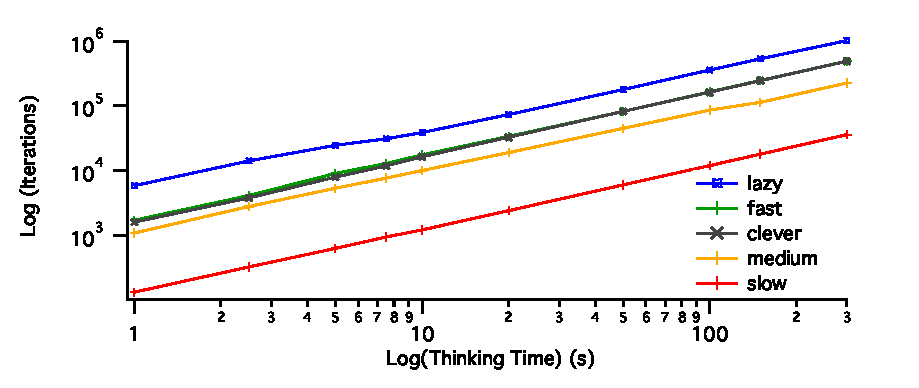
\includegraphics{thinking2.eps}}
\caption{Number of {MCTS} iterations performed to decide first move when starting from an empty $12\times 12$ board. Plotted against thinking time.}
\label{fig:linear}
\end{figure}

Figure \ref{fig:linear} shows that the number of iterations performed on the first move is directly proportional to the thinking time allocated for the first move. This is unsurpring for the {Slow}, {Medium}, {Fast}, and {Clever} agents. For these agents, every iteration represents performing a full Simulation from a start node to termination. It is a surprising result for the {Lazy} agent. In the {Lazy} agent, as more Simulations are performed, the tree grows, but only a maximum of 10 nodes are simulated beyond the fringe of the tree. From this, one would expect that the number of iterations performed per unit thinking time would decrease as the tree grows in size. Figure \ref{fig:linear} shows that this effect does not occur, at least for trees containing up to a million nodes. This suggests the Selection and Backpropagation phases are not a significant contribution to overhead, when compared to the Simulation and Expansion phases. Profiling data generated by the {Lazy} agent supported these findings.

\begin{figure}
\centering
{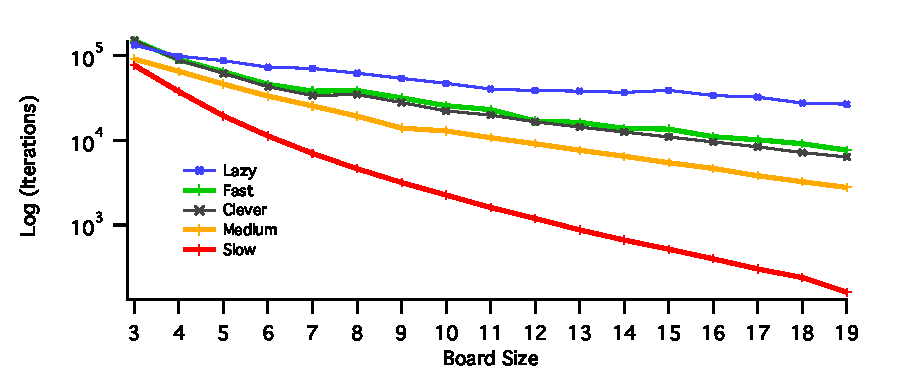
\includegraphics{boardsizeiter.eps}}
\caption{Number of {MCTS} iterations performed in 10 seconds to decide first move when starting from an empty board. Plotted against board size.\label{fig:boardsize}}
\end{figure}

Figure \ref{fig:boardsize} shows that all agents are roughly the same for small board sizes. This is unsuprising since {MCTS} quickly builds the entire game tree when the state space is small. For example, in the case of $3 \times 3$ boards, after about 1000 iterations the full game tree is built, and the rest of the work performed by the agent is repeated Selection. The Selection phase is implemented in the same way for all of the agents. 

The number of iterations performed decreases dramatically for all agents as the board size increases. This is to be expected since increasing board size increases both the branching factor at each move and the average depth at which Simulations terminate. The {Lazy} agent is affected least by the board size since the average depth at which Simulations terminate is always 10, regardless of board size.

The points in Figure \ref{fig:boardsize} for the {Lazy}, {Fast}, {Clever}and {Medium} agents look unreliable since they don't appear to fit a curve well. Repeated trials showed that the standard deviations for all points were at most $0.1\%$ of their corresponding mean values. The slightly erratic behaviour may be due to the idiosyncrasies of different board-sizes. In Figure \ref{fig:boardsize}, on a board size of 12 the {Clever} and {Fast} agents perform almost the exact same number of iterations as each other when given 10 seconds thinking time. Figure \ref{fig:linear} shows that this observation holds across a range of thinking times for $12 \times 12$ boards. 

In general, the {Clever} agent performs almost as well as the {Fast} agent. This strongly suggests that the {WinSave} heuristic contributes very little to the overall overhead of the search.



\subsection{{Connect}(12,12,5,1,1) Tournament Performance}

\begin{figure}
\centering
{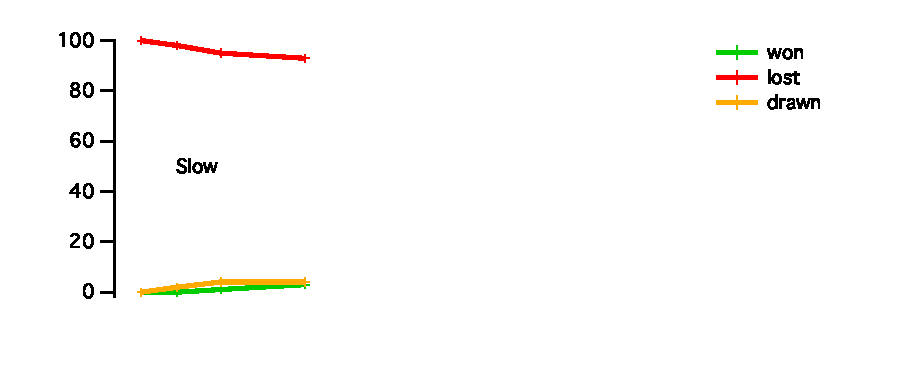
\includegraphics{slowwld.eps}}
{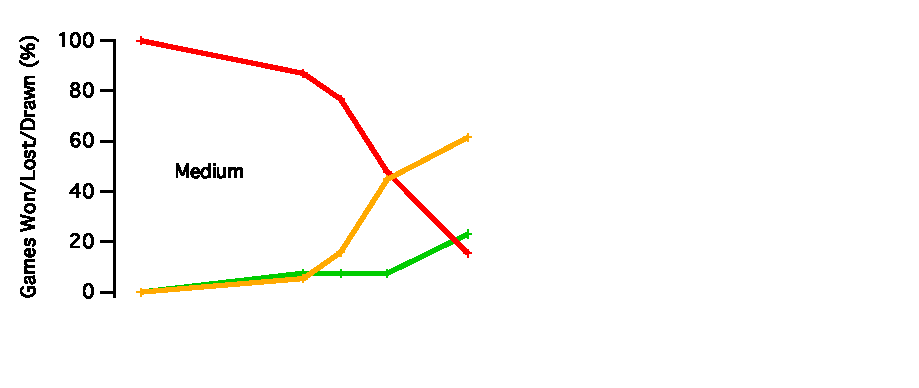
\includegraphics{medwld.eps}}
{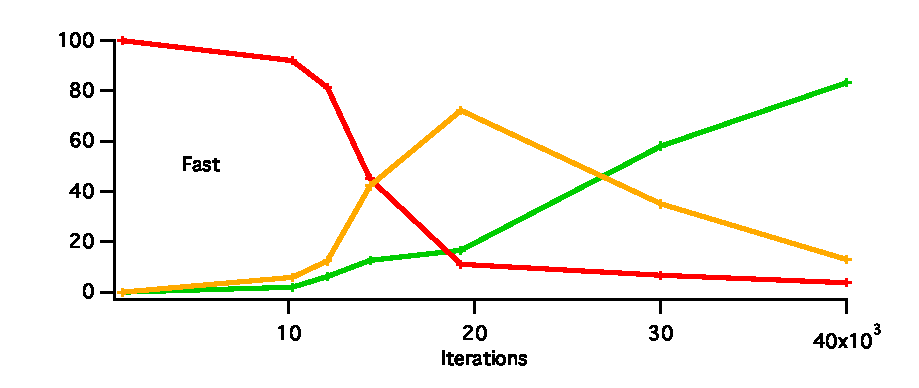
\includegraphics{fastwld.eps}}
\caption{Tournament results for the {Slow}, {Medium}, and {Fast} agents. Each plays against the {Threats} utility function with modest minimax search. The tournament results are plotted against the average number of iterations performed for the first move in each game.}
\label{fig:wld}
\end{figure}

Figure \ref{fig:wld} shows that, when the {Fast}, {Medium} and {Slow} agents are able to perform the same number of iterations on their first move, the three agents perform similarly in tournaments. This is consistent with the fact that {Fast}, {Medium} and {Slow} perform {MCTS} in exactly the same way, the only difference being their efficiency (see informal proof in Section \ref{sec:informal_proof}). The {Slow} and {Medium} agents are not plotted for the full $x$ axis due to Simulation time constraints. For example, a single 100 game tournament for the {Slow} agent for an $x$ value of 40,000, would take approximately 33 hours.

Figure \ref{fig:wld} also shows three approximate phases of tournament performance: for 0-15 thousand iterations, most games are lost; for 15-27 thousand iterations, most games are drawn; and for more than 27 thousand iterations, most games are won. Qualitive analysis of games played show two sub phases in the 0-15 thousand range: for 0-8 thousand iterations, most moves seem irrational and essentially random; for 8-15 thousand iterations, most moves are sensible but the agent is outplayed by the stronger {Threats} agent. 

\begin{figure}
\centering
{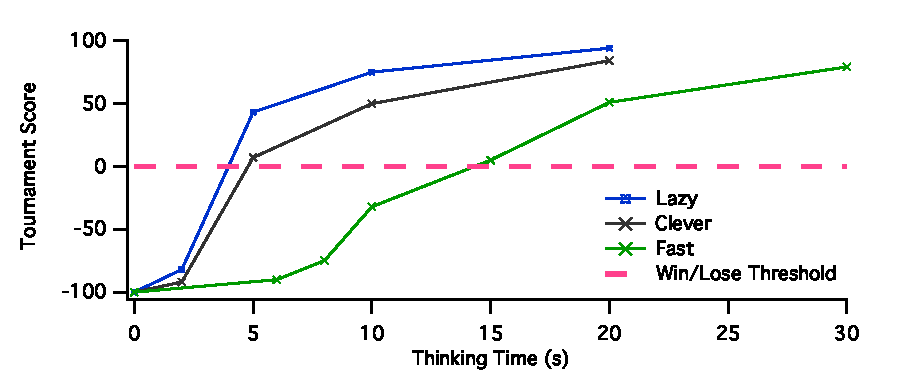
\includegraphics{thinking.eps}}
\caption{The tournament results plotted against thinking time.}
\label{fig:results}
\end{figure}

Figure \ref{fig:results} shows that, for any given thinking time, the most successful agents are {Lazy}, {Clever} and {Fast} in that order. {Slow} and {Medium} are not considered as they perform {MCTS} in the same fashion as {Fast}, but at a slower speed. The fact that {Clever} performs better than {Fast} is to be expected; the {WinSave} heuristic has runtime performance almost as good as {Fast}, but has a more rational tree and Simulation policy. The fact that {Lazy} performs better than {Clever} is interesting: for $12 \times 12$ boards, the boost in speed performance from terminating Simulations early outweighs the loss in tournament performance per iteration. Figure \ref{fig:boardsize} suggests that as boards get larger, the advantages of using {Lazy} over {Clever} increase.



\subsection{{Connect}(13,13,6,2,1) Tournament Performance}
No agents are able to play {Connect}(13,13,6,2,1) well against the {Threats} utility function, even when given up to 300 seconds thinking-time for each turn. The {Clever} agent is able to perform reasonably well against a random agent. However qualitive analysis of these games show that the {Clever} agent will play randomly until a win that turn is possible, or it is forced to block that turn. These results could be due to the high branching factor of {Connect}(13,13,6,2,1), $\binom{13 \times 13 -1}{2} = 20856$. This is about 145 times higher than the branching factor for {Connect}(12,12,5,1,1). The {Lazy} agent, which performs one million iterations in 300 seconds, would only be able to dedicate an average of 50 iterations to each of the possible moves within this time. This problem was foreseen during development, and as such, each ply of the game tree does not represent a single turn, but a single move. This reduces the branching factor in the tree to the `move' branching factor, 169. This result shows that this was not sufficient to solve the problem.

\subsection{{Freestyle GoMoku} and {Connect6} Tournaments}
The {Lazy} agent was chosen for the {Freestyle GoMoku} tournament since it outplays {Clever} for $12 \times 12$ boards. The number of iterations performed by {Lazy} on $15 \times 15$ boards is a slight increase on $12 \times 12$ boards. In contrast, the number of iterations performed by {Clever} from $12 \times 12$ to $15 \times 15$ boards drops by $40\%$. 

The tournament was played against the \text{Threats} utility function with modest search parameters. The {Lazy} agent won the tournament, winning $31\%$ of the games. The narrow margin of this win highlights the scalability issues for the {MCTS} agent. While the tournament performance of {Threats} with minimax search is fairly constant as board size increases, the performance of the {MCTS} agent deteriorates rapidly. Not only can fewer iterations be performed on larger boards, but more iterations are required to play well. It was not considered worthwhile running a {Connect6} tournament.

%Figure \ref{fig:wld}, \r shows this agent is fairly hopeless. The results for 100 seconds of thinking time are promising since it suggests there is nothing fundamentally wrong with the agent, but it needs to be made faster. Indeed, qualitative analysis shows game strategy gradually improves as more thinking time is permitted per move. The number of iterations performed increases linearly with thinking time. This suggests the main bulk of the work done in the {Simulation} phase and not the tree phases of the search. This is consistent with the profiling data gathered for this agent.

%Figure \ref{fig:slow313} shows the number of simulations which can be performed is inversely proportional to the ...









